\documentclass[12pt,a4paper]{article}
\usepackage[legalpaper, portrait, margin=2cm]{geometry}
\usepackage[export]{adjustbox}
\usepackage{amsmath}
\usepackage{fancyhdr}
\usepackage{hyperref}
\usepackage{listings}
\usepackage{xcolor}
\usepackage{setspace}
\usepackage{enumitem}
\newcommand{\subscript}[2]{$#1 _ #2$}

\onehalfspacing
\addtolength\jot{8pt}

\graphicspath{ {./docs/} }


\hypersetup{
	citecolor=blue,
	colorlinks=true,
	filecolor=magenta,
	linkcolor=blue,
	pdfpagemode=FullScreen,
	pdftitle={Homework III - Group 67},
	urlcolor=blue,
}

\lstdefinestyle{Python}{
	basicstyle=\footnotesize\ttfamily,
	frame=single,
	keywordstyle=\color{red},
	numbers=left,
	numbersep=5pt,
	numberstyle=\tiny\color{gray},
	showspaces=false,
	showstringspaces=false,
	showtabs=false,
	stringstyle=\color{blue},
	tabsize=4
}

\lstset{style=Python}

\pagestyle{fancy}
\fancyhf{}
\rhead{Grupo \textbf{67}}
\lhead{Aprendizagem 2022/23 - Homework III}
\cfoot{Luís Câmara (99099) e Pedro Lobo (99115)}

\renewcommand{\thesection}{\Roman{section}}
\renewcommand{\thesubsection}{\arabic{subsection}}

\newcommand{\X}{
	\begin{bmatrix}
		1 & 0.8 & 0.64 & 0.512 \\
		1 & 1   & 1    & 1     \\
		1 & 1.2 & 1.44 & 1.728 \\
		1 & 1.4 & 1.96 & 2.744 \\
		1 & 1.6 & 2.56 & 4.096
	\end{bmatrix}
}

\newcommand{\Xone}{
	\begin{bmatrix}
		1 & 0.8 & 0.64 & 0.512
	\end{bmatrix}
}

\newcommand{\Xtwo}{
	\begin{bmatrix}
		1 & 1 & 1 & 1
	\end{bmatrix}
}

\newcommand{\Xthree}{
	\begin{bmatrix}
		1 & 1.2 & 1.44 & 1.728
	\end{bmatrix}
}

\newcommand{\Xfour}{
	\begin{bmatrix}
		1 & 1.4 & 1.96 & 2.744
	\end{bmatrix}
}

\newcommand{\Xfive}{
	\begin{bmatrix}
		1 & 1.6 & 2.56 & 4.096
	\end{bmatrix}
}

\newcommand{\z}{
	\begin{bmatrix}
		24 \\
		20 \\
		10 \\
		13 \\
		12
	\end{bmatrix}
}

\newcommand{\w}{
	\begin{bmatrix}
		\wzero & \wone & \wtwo & \wthree
	\end{bmatrix}
}

\newcommand{\wzero}{
	7.0450759
}

\newcommand{\wone}{
	4.64092765
}

\newcommand{\wtwo}{
	1.96734046
}

\newcommand{\wthree}{
	-1.30088142
}

\newcommand{\wnormsq}{
	76.73402482370348
}

\newcommand{\error}{
	46.83068498017306
}

\newcommand{\rmse}{
	6.843294892094967
}

\newcommand{\wT}{
	\begin{bmatrix}
		\wzero  \\
		\wone   \\
		\wtwo   \\
		\wthree \\
	\end{bmatrix}
}

\newcommand{\wonefirst} {
	\begin{bmatrix}
		1 \\
		1
	\end{bmatrix}
}

\newcommand{\azerofirst} {
	0.8
}

\newcommand{\bonefirst} {
	\begin{bmatrix}
		1 \\
		1
	\end{bmatrix}
}

\newcommand{\netonefirst} {
	\begin{bmatrix}
		1.8 \\
		1.8
	\end{bmatrix}
}

\newcommand{\aonefirst} {
	\begin{bmatrix}
		1.19721736 \\
		1.19721736
	\end{bmatrix}
}

\newcommand{\wtwofirst} {
	\begin{bmatrix}
		1 & 1
	\end{bmatrix}
}

\newcommand{\btwofirst} {
	1
}

\newcommand{\atwofirst} {
	1.404166
}

\newcommand{\nettwofirst} {
	3.3944347262436203
}

\newcommand{\latwofirst} {
	-22.595834083700154
}

\newcommand{\atwonettwofirst} {
	0.1404165916299847
}

\newcommand{\nettwoaonefirst} {
	\begin{bmatrix}
		1 \\
		1
	\end{bmatrix}
}

\newcommand{\aonenetonefirst} {
	\begin{bmatrix}
		0.11972174 & 0 \\
		0 & 0.11972174
	\end{bmatrix}
}

\newcommand{\deltatwofirst} {
	-3.1728300070698143
}

\newcommand{\deltaonefirst} {
	\begin{bmatrix}
		-0.37985672 \\
		-0.37985672
	\end{bmatrix}
}

\newcommand{\lbtwofirst} {
	\deltatwofirst
}

\newcommand{\lbonefirst} {
	\deltaonefirst
}

\newcommand{\lwtwofirst} {
	\begin{bmatrix}
		-3.79856717 & -3.79856717
	\end{bmatrix}
}

\newcommand{\lwonefirst} {
	\begin{bmatrix}
		-0.30388537 \\
		-0.30388537
	\end{bmatrix}
}

\newcommand{\wonesecond} {
	\begin{bmatrix}
		1 \\
		1
	\end{bmatrix}
}

\newcommand{\azerosecond} {
	1
}

\newcommand{\bonesecond} {
	\begin{bmatrix}
		1 \\
		1
	\end{bmatrix}
}

\newcommand{\netonesecond} {
	\begin{bmatrix}
		2 \\
		2
	\end{bmatrix}
}

\newcommand{\aonesecond} {
	\begin{bmatrix}
		1.22140276 \\
		1.22140276
	\end{bmatrix}
}

\newcommand{\wtwosecond} {
	\begin{bmatrix}
		1 & 1
	\end{bmatrix}
}

\newcommand{\btwosecond} {
	1
}

\newcommand{\atwosecond} {
	1.410974431163945
}

\newcommand{\nettwosecond} {
	3.4428055163203397
}

\newcommand{\latwosecond} {
	-18.589025568836057
}

\newcommand{\atwonettwosecond} {
	0.1410974431163945
}

\newcommand{\nettwoaonesecond} {
	\begin{bmatrix}
		1 \\
		1
	\end{bmatrix}
}

\newcommand{\aonenetonesecond} {
	\begin{bmatrix}
		0.12214028 & 0 \\
		0 & 0.12214028
	\end{bmatrix}
}

\newcommand{\deltatwosecond} {
	-2.6228639777880485
}

\newcommand{\deltaonesecond} {
	\begin{bmatrix}
		-0.32035733 \\
		-0.32035733
	\end{bmatrix}
}

\newcommand{\lbtwosecond} {
	\deltatwosecond
}

\newcommand{\lbonesecond} {
	\deltaonesecond
}

\newcommand{\lwtwosecond} {
	\begin{bmatrix}
		-3.2035733 & -3.2035733
	\end{bmatrix}
}

\newcommand{\lwonesecond} {
	\begin{bmatrix}
		-0.32035733 \\
		-0.32035733
	\end{bmatrix}
}

\newcommand{\wonethird} {
	\begin{bmatrix}
		1 \\
		1
	\end{bmatrix}
}

\newcommand{\azerothird} {
	1.2
}

\newcommand{\bonethird} {
	\begin{bmatrix}
		1 \\
		1
	\end{bmatrix}
}

\newcommand{\netonethird} {
	\begin{bmatrix}
		2.2 \\
		2.2
	\end{bmatrix}
}

\newcommand{\aonethird} {
	\begin{bmatrix}
		1.24607673 \\
		1.24607673
	\end{bmatrix}
}

\newcommand{\wtwothird} {
	\begin{bmatrix}
		1 & 1
	\end{bmatrix}
}

\newcommand{\btwothird} {
	1
}

\newcommand{\atwothird} {
	1.4179545084644258
}

\newcommand{\nettwothird} {
	3.4921534611747616
}

\newcommand{\latwothird} {
	-8.582045491535574
}

\newcommand{\atwonettwothird} {
	0.1417954508464426
}

\newcommand{\nettwoaonethird} {
	\begin{bmatrix}
		1 \\
		1
	\end{bmatrix}
}

\newcommand{\aonenetonethird} {
	\begin{bmatrix}
		0.12460767 & 0 \\
		0 & 0.12460767
	\end{bmatrix}
}

\newcommand{\deltatwothird} {
	-1.2168950096569668
}

\newcommand{\deltaonethird} {
	\begin{bmatrix}
		-0.15163446 \\
		-0.15163446
	\end{bmatrix}
}

\newcommand{\lbtwothird} {
	\deltatwothird
}

\newcommand{\lbonethird} {
	\deltaonethird
}

\newcommand{\lwtwothird} {
	\begin{bmatrix}
		-1.51634456 & -1.51634456
	\end{bmatrix}
}

\newcommand{\lwonethird} {
	\begin{bmatrix}
		-0.18196135 \\
		-0.18196135
	\end{bmatrix}
}

\newcommand{\btwonew} {
	1.701258899451483
}

\newcommand{\bonenew} {
	\begin{bmatrix}
		1.08518485 \\
		1.08518485
	\end{bmatrix}
}

\newcommand{\wtwonew} {
	\begin{bmatrix}
		1.8518485 & 1.8518485
	\end{bmatrix}
}

\newcommand{\wonenew} {
	\begin{bmatrix}
		1.08062041 \\
		1.08062041
	\end{bmatrix}
}

\newcommand{\ridgemae} {
	0.162829976437694
}

\newcommand{\mlponemae} {
	0.0680414073796843
}

\newcommand{\mlptwomae} {
	0.0978071820387748
}

\newcommand{\mlponeiterations} {
	452
}

\newcommand{\mlptwoiterations} {
	77
}

\begin{document}

\section{Pen-and-paper}
\begin{enumerate}
	\item
	      \begin{tabular}[t]{|c|c|c|c|c|}
	      	\hline
	      	      & $y_1$ & $y_1^2$ & $y_1^3$ \\
	      	\hline
	      	$x_1$ & 0.8   & 0.64    & 0.512   \\
	      	\hline
	      	$x_2$ & 1     & 1       & 1       \\
	      	\hline
	      	$x_3$ & 1.2   & 1.44    & 1.728   \\
	      	\hline
	      	$x_4$ & 1.4   & 1.96    & 2.744   \\
	      	\hline
	      	$x_5$ & 1.6   & 2.56    & 4.096   \\
	      	\hline
	      \end{tabular}

	      \begin{flalign*}
	      	w & = (X^T \cdot X + \lambda I)^{-1} \cdot X^T \cdot z          &\\
	      	  & = \left(\X^T \cdot \X + 2I \right)^{-1} \cdot \X^T \cdot \z &\\
			  & = \left(\begin{bmatrix} 5 & 6 & 7.6 & 10.08 \\ 6 & 7.6 & 10.08 & 13.8784 \\ 7.6 & 10.08 & 13.8784 & 19.68 \\ 10.08 & 13.8784 & 19.68 & 28.55488 \end{bmatrix} + 2I \right)^{-1} \cdot \X^T \cdot \z &\\
			  & = \left(\begin{bmatrix} 7 & 6 & 7.6 & 10.08 \\ 6 & 9.6 & 10.08 & 13.8784 \\ 7.6 & 10.08 & 15.8784 & 19.68 \\ 10.08 & 13.8784 & 19.68 & 30.55488 \\ \end{bmatrix} \right)^{-1} \cdot \X^T \cdot \z &\\
			  & = \begin{bmatrix} 0.34168753 & -0.1214259 & -0.07490231 & -0.00932537 \\ -0.1214259 & 0.3892078 & -0.09667718 & -0.07445624 \\ -0.07490231 & -0.09667718 & 0.37257788 & -0.17135047 \\ -0.00932537 & -0.07445624 & -0.17135047 & 0.17998796 \\ \end{bmatrix} \cdot \X^T \cdot \z &\\
				  & = \begin{bmatrix} 0.19183474 & 0.13603395 & 0.07200288 & -0.00070608 & -0.08254055 \\ 0.08994535 & 0.09664848 & 0.07774793 & 0.02966982 & -0.05115977 \\ -0.00152564 & 0.02964793 & 0.04950363 & 0.04981662 & 0.02236208 \\ -0.08640083 & -0.07514413 & -0.03439835 & 0.04447593 & 0.17011812 \\ \end{bmatrix} \cdot \z &\\
	      	  & = \wT
	      \end{flalign*}

	      \pagebreak

	\item
	      \begin{flalign*}
			  E & = \frac{1}{5} \sum_{i=1}^{5}(z_i - \hat{z_i})^2       &\\
	      	     & = \frac{1}{5} \left[ \left(24 - \wT \cdot \Xone \right)^2 \right.                    &\\
	      	     & \hskip1.7em\relax \left. + \left(20 - \wT \cdot \Xtwo \right)^2            \right.                     &\\
	      	     & \hskip1.7em\relax \left. + \left(10 - \wT \cdot \Xthree \right)^2          \right.                     &\\
	      	     & \hskip1.7em\relax \left. + \left(13 - \wT \cdot \Xfour \right)^2           \right.                     &\\
	      	     & \hskip1.7em\relax \left. + \left(12 - \wT \cdot \Xfive \right)^2 \right] &\\
	      	     & = \error
	      \end{flalign*}
	      \begin{flalign*}
	      	\text{RMSE} = \sqrt{E} = \sqrt{\error} = \rmse
	      \end{flalign*}

	      \pagebreak

	\item

	      \begin{enumerate}[label=\subscript{x}{{\arabic*}})]
	      	\item
				\begin{itemize}
					\item Forward Propagation
	      	      \begin{flalign*}
	      	      	& \text{net}^{[1]} = w^{[1]} \cdot a^{[0]} + b^{[1]} = \wonefirst \times \azerofirst + \bonefirst = \netonefirst &&\\
				    & \text{a}^{[1]} = e^{0.1 \times \text{net}^{[1]}} = \aonefirst &&\\
	      	      	& \text{net}^{[2]} = w^{[2]} \cdot a^{[1]} + b^{[2]} = \wtwofirst \cdot \aonefirst + \btwofirst = \nettwofirst &&\\
	      	      	& \text{a}^{[2]} = e^{0.1 \times \text{net}^{[2]}} = \atwofirst &&\\
				  \end{flalign*}

			  \item Backward Propagation
					\begin{flalign*}
	      	      	& \dfrac{\partial l}{\partial a^{[2]}} = a^{[2]} - z = \latwofirst &&\\
						& \dfrac{\partial a^{[2]}}{\partial \text{net}^{[2]}} = 0.1 \times e^{0.1 \times \text{net}^{[2]}} = \atwonettwofirst &&\\
	      	      	& \dfrac{\partial \text{net}^{[2]}}{\partial a^{[1]}} = (w^{[2]})^T = \nettwoaonefirst &&\\
						& \dfrac{\partial \text{a}^{[1]}}{\partial \text{net}^{[1]}} = \begin{bmatrix} 0.1 \times e^{0.1 \times \text{net}_1^{[1]}} & 0 \\ 0 & 0.1 \times e^{0.1 \times \text{net}_2^{[1]}} \end{bmatrix} = \aonenetonefirst &&\\
	      	      	& \delta^{[2]} = \dfrac{\partial l}{\partial \text{net}^{[2]}} = \dfrac{\partial a^{[2]}}{\partial \text{net}^{[2]}} \cdot \dfrac{\partial l}{\partial \text{a}^{[2]}} = \deltatwofirst &&\\
	      	      	& \delta^{[1]} = \dfrac{\partial l}{\partial \text{net}^{[1]}} = \dfrac{\partial a^{[1]}}{\partial \text{net}^{[1]}} \cdot \dfrac{\partial \text{net}^{[2]}}{\partial \text{a}^{[1]}} \times \delta^{[2]} = \deltaonefirst &&\\
	      	      	& \dfrac{\partial l}{\partial b^{[2]}} = \delta^{[2]} = \lbtwofirst &&\\
	      	      	& \dfrac{\partial l}{\partial b^{[1]}} = \delta^{[1]} = \lbonefirst &&\\
	      	      	& \dfrac{\partial l}{\partial w^{[2]}} = \delta^{[2]} \cdot (a^{[1]})^T = \lwtwofirst &&\\
	      	      	& \dfrac{\partial l}{\partial w^{[1]}} = \delta^{[1]} \cdot x^T = \lwonefirst &
	      	      \end{flalign*}
				\end{itemize}

			\pagebreak

	      	\item
				\begin{itemize}
					\item Forward Propagation
	      	      \begin{flalign*}
	      	      	& \text{net}^{[1]} = w^{[1]} \cdot a^{[0]} + b^{[1]} = \wonesecond \times \azerosecond + \bonesecond = \netonesecond  &\\
	      	      	& \text{a}^{[1]} = e^{0.1 \times \text{net}^{[1]}} = \aonesecond  &\\
	      	      	& \text{net}^{[2]} = w^{[2]} \cdot a^{[1]} + b^{[2]} = \wtwosecond \cdot \aonesecond + \btwosecond = \nettwosecond  &\\
	      	      	& \text{a}^{[2]} = e^{0.1 \times \text{net}^{[2]}} = \atwosecond\ &\\
				  \end{flalign*}

			  \item Backward Propagation
						\begin{flalign*}
	      	      	& \dfrac{\partial l}{\partial a^{[2]}} = a^{[2]} - z = \latwosecond  &\\
							& \dfrac{\partial a^{[2]}}{\partial \text{net}^{[2]}} = 0.1 \times e^{0.1 \times \text{net}^{[2]}} = \atwonettwosecond  &\\
	      	      	& \dfrac{\partial \text{net}^{[2]}}{\partial a^{[1]}} = (w^{[2]})^T = \nettwoaonesecond  &\\
					& \dfrac{\partial \text{a}^{[1]}}{\partial \text{net}^{[1]}} = \begin{bmatrix} 0.1 \times e^{0.1 \times \text{net}_1^{[1]}} & 0 \\ 0 & 0.1 \times e^{0.1 \times \text{net}_2^{[1]}} \end{bmatrix} = \aonenetonesecond  &\\
	      	      	& \delta^{[2]} = \dfrac{\partial l}{\partial \text{net}^{[2]}} = \dfrac{\partial a^{[2]}}{\partial \text{net}^{[2]}} \cdot \dfrac{\partial l}{\partial \text{a}^{[2]}} = \deltatwosecond  &\\
	      	      	& \delta^{[1]} = \dfrac{\partial l}{\partial \text{net}^{[1]}} = \dfrac{\partial a^{[1]}}{\partial \text{net}^{[1]}} \cdot \dfrac{\partial \text{net}^{[2]}}{\partial \text{a}^{[1]}} \times \delta^{[2]} = \deltaonesecond &\\
	      	      	& \dfrac{\partial l}{\partial b^{[2]}} = \delta^{[2]} = \lbtwosecond  &\\
	      	      	& \dfrac{\partial l}{\partial b^{[1]}} = \delta^{[1]} = \lbonesecond  &\\
	      	      	& \dfrac{\partial l}{\partial w^{[2]}} = \delta^{[2]} \cdot (a^{[1]})^T = \lwtwosecond  &\\
	      	      	& \dfrac{\partial l}{\partial w^{[1]}} = \delta^{[1]} \cdot x^T = \lwonesecond
	      	      \end{flalign*}
				\end{itemize}

			\pagebreak

	      	\item
				\begin{itemize}
					\item Forward Propagation
	      	      \begin{flalign*}
	      	      	& \text{net}^{[1]} = w^{[1]} \cdot a^{[0]} + b^{[1]} = \wonethird \times \azerothird + \bonethird = \netonethird  &\\
	      	      	& \text{a}^{[1]} = e^{0.1 \times \text{net}^{[1]}} = \aonethird  &\\
	      	      	& \text{net}^{[2]} = w^{[2]} \cdot a^{[1]} + b^{[2]} = \wtwothird \cdot \aonethird + \btwothird = \nettwothird  &\\
	      	      	& \text{a}^{[2]} = e^{0.1 \times \text{net}^{[2]}} = \atwothird\ &\\
				  \end{flalign*}

			  \item Backward Propagation
				  \begin{flalign*}
	      	      	& \dfrac{\partial l}{\partial a^{[2]}} = a^{[2]} - z = \latwothird  &\\
					& \dfrac{\partial a^{[2]}}{\partial \text{net}^{[2]}} = 0.1 \times e^{0.1 \times \text{net}^{[2]}} = \atwonettwothird  &\\
	      	      	& \dfrac{\partial \text{net}^{[2]}}{\partial a^{[1]}} = (w^{[2]})^T = \nettwoaonethird  &\\
    				& \dfrac{\partial \text{a}^{[1]}}{\partial \text{net}^{[1]}} = \begin{bmatrix} 0.1 \times e^{0.1 \times \text{net}_1^{[1]}} & 0 \\ 0 & 0.1 \times e^{0.1 \times \text{net}_2^{[1]}} \end{bmatrix} = \aonenetonethird  &\\
	      	      	& \delta^{[2]} = \dfrac{\partial l}{\partial \text{net}^{[2]}} = \dfrac{\partial a^{[2]}}{\partial \text{net}^{[2]}} \cdot \dfrac{\partial l}{\partial \text{a}^{[2]}} = \deltatwothird  &\\
	      	      	& \delta^{[1]} = \dfrac{\partial l}{\partial \text{net}^{[1]}} = \dfrac{\partial a^{[1]}}{\partial \text{net}^{[1]}} \cdot \dfrac{\partial \text{net}^{[2]}}{\partial \text{a}^{[1]}} \times \delta^{[2]} = \deltaonethird &\\
	      	      	& \dfrac{\partial l}{\partial b^{[2]}} = \delta^{[2]} = \lbtwothird  &\\
	      	      	& \dfrac{\partial l}{\partial b^{[1]}} = \delta^{[1]} = \lbonethird  &\\
	      	      	& \dfrac{\partial l}{\partial w^{[2]}} = \delta^{[2]} \cdot (a^{[1]})^T = \lwtwothird  &\\
	      	      	& \dfrac{\partial l}{\partial w^{[1]}} = \delta^{[1]} \cdot x^T = \lwonethird
	      	      \end{flalign*}
				\end{itemize}

	      \end{enumerate}

		  \pagebreak

		  \begin{itemize}
			  \item Batch Gradient Descent Update
	      \begin{flalign*}
			  b^{[2]} & = b^{[2]} - \eta \sum_{i=1}^{3} \dfrac{\partial l}{\partial b^{[2]}}      &\\
					& = \btwofirst - 0.1 \left(\lbtwofirst + \lbtwosecond + \lbtwothird \right) &\\
	      	        & = \btwonew
	      \end{flalign*}

	      \begin{flalign*}
	      	b^{[1]} & = b^{[1]} - \eta \sum_{i=1}^{3} \dfrac{\partial l}{\partial b^{[1]}}      &\\
	      	        & = \bonefirst - 0.1 \left(\lbonefirst + \lbonesecond + \lbonethird \right) &\\
	      	        & = \bonenew
	      \end{flalign*}

	      \begin{flalign*}
	      	w^{[2]} & = w^{[2]} - \eta \sum_{i=1}^{3} \dfrac{\partial l}{\partial w^{[2]}}     &\\
					& = \wtwofirst - 0.1 \left(\lwtwofirst + \right. &\\
					& \hskip7.2em\relax \left. \lwtwosecond + \right. &\\
					& \hskip7.2em\relax \left. \lwtwothird \right) &\\
	      	        & = \wtwonew
	      \end{flalign*}

	      \begin{flalign*}
	      	w^{[1]} & = w^{[1]} - \eta \sum_{i=1}^{3} \dfrac{\partial l}{\partial w^{[1]}}     &\\
	      	        & = \wonefirst - 0.1 \left(\lwonefirst + \lwonesecond + \lwonethird\right) &\\
	      	        & = \wonenew
	      \end{flalign*}
		  \end{itemize}

\end{enumerate}

\pagebreak

\section{Programming}

\begin{enumerate}[resume]
	\item
	      Ridge MAE = $\ridgemae$ \\
	      MLP1 MAE =  $\mlponemae$ \\
	      MLP2 MAE = $\mlptwomae$

	      \pagebreak

	\item \mbox{}
	      \begin{figure}[h]
	      	\centering
	      	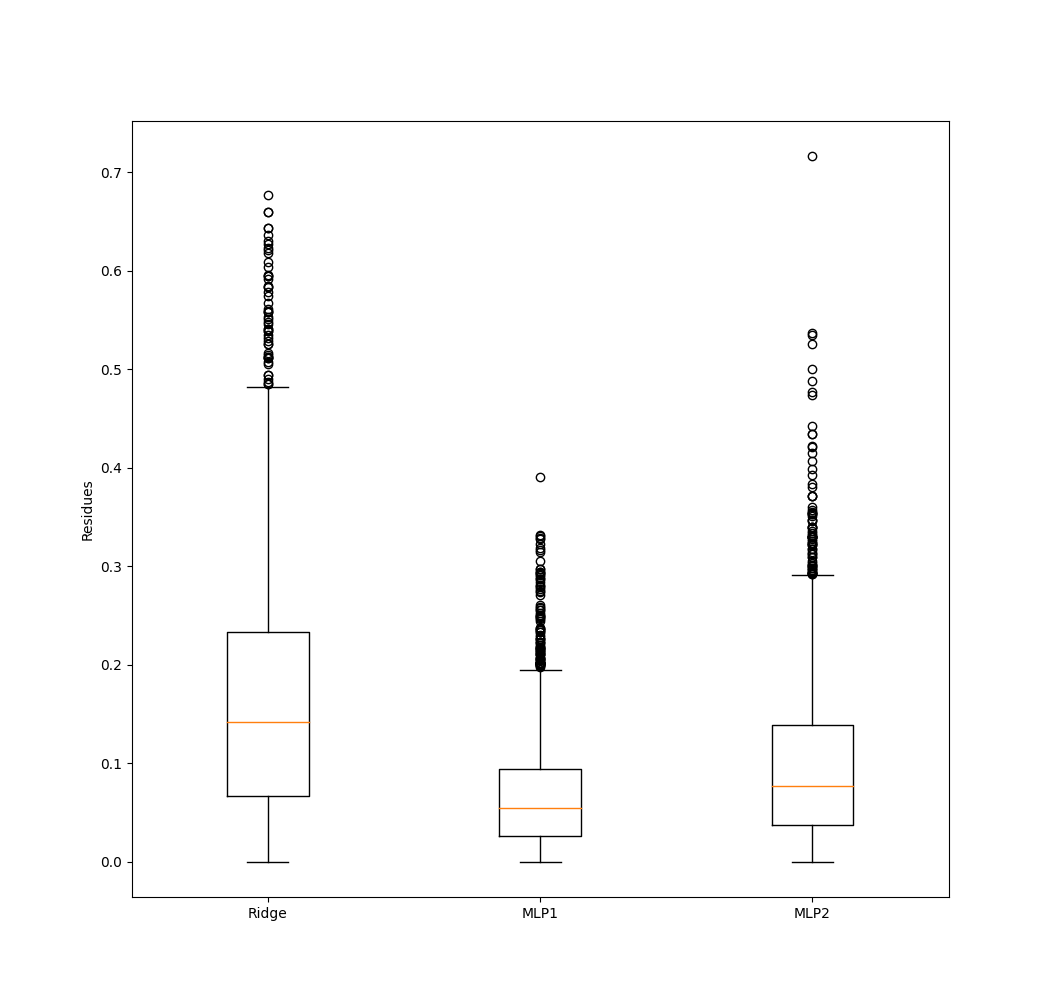
\includegraphics[scale=0.45,valign=t]{boxplot}
	      	\caption{Boxplot}
	      	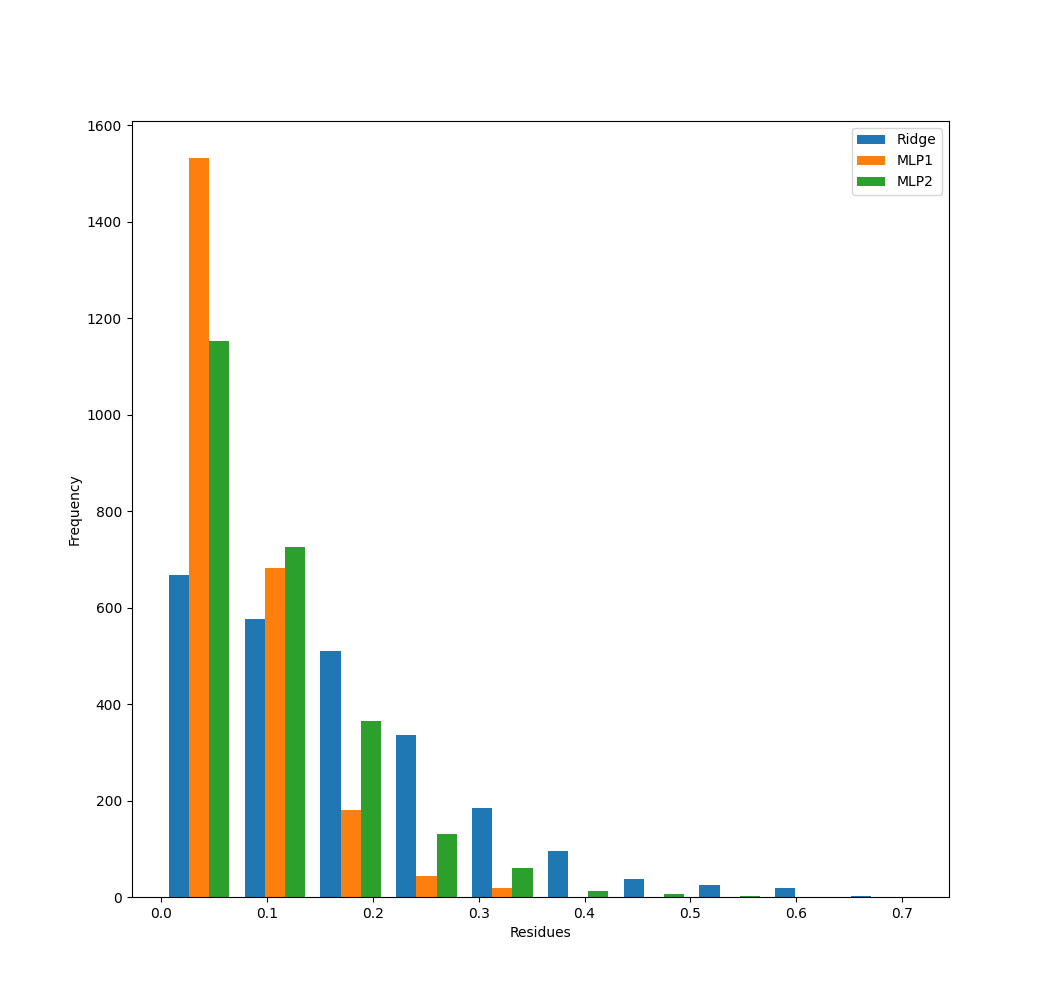
\includegraphics[scale=0.45,valign=t]{hist}
	      	\caption{Histogram}
	      \end{figure}

	      \pagebreak

	\item
	      The MLP1 converged in $\mlponeiterations$ iterations. \\
	      The MLP2 converged in $\mlptwoiterations$ iterations.

	\item
		The two MLP differ in the stopping criteria. The MLP1 sets
		aside 10\% of the training data as validation, terminating when
		the validation score doesn't improve significantly for some
		number of consecutive epochs.  The MLP2 terminates when the
		training loss does not improve for some number of consecutive
		epochs.

		The training loss function converges faster than the validation
		score.  The MLP2 goes through the training set, fitting to it
		rather quickly.  Therefore, the training loss converges after
		few iterations, not improving by much between epochs,
		triggering the training termination. On the other hand, the
		MLP1 is confronted with the validation set. The validation
		score converges slowly as the MLP1 is confronted with data that
		it didn't yet observed.

		The gathered results support this conclusion, as the MLP2
		performs better in the testing set, relative to the MLP1.
		Therefore, the MLP1, despite fitting better to the training
		set, performs poorly on the testing set.  Therefore, MLP1
		suffers from overfitting.

\end{enumerate}

\pagebreak

\section{Appendix}
\lstinputlisting[language=Python]{./src/code.py}

\end{document}
